\documentclass[dvipdfmx]{jsarticle}
\usepackage[final]{graphicx}

% 数式
\usepackage{amsmath,amsfonts}
\usepackage{bm}
% 画像

\include{setting.txt}


\begin{document}

\title{スタックの実装と応用}
\author{古城隆人}
\date{\today}
\maketitle

% \tableofcontents

\newpage


\section{目的}
ススタックを用いたデータ構造を理解し、スタックを用いたプログラムを作成することで、スタックの基本的な操作を理解する。また、スタックを用いたハノイの塔のプログラムを作成し、理解を深める。
\section{原理}
\subsection{スタック}
スタックとはデータ構造の一種であり、データの追加や削除が限定的に行うことが出来る構造である。
限定的にすることによりデータの数が増えてもデータの挿入や削除にかかる時間が一定になるという利点がある。
スタックはデータが出入りする順番により、LIFO(Last In First Out)、FILO(First in Last out)と呼ばれる。
スタックには以下の操作がある。
\begin{itemize}
  \item push: スタックにデータを追加する
  \item pop: スタックからデータを取り出す
\end{itemize}
pushを行うと、スタックの一番上にデータが追加される。
popを行うと、スタックの一番上のデータが取り出され、取り出したデータを削除する。
\subsection{ハノイの塔}\label{sec:mysection}
ハノイの塔は、3本の杭とその上に積まれた円盤からなるパズルである。移動のルールは以下の通りである。
\begin{itemize}
  \item 1回の移動で1枚の円盤しか動かせない
  \item 小さい円盤の上に大きい円盤を乗せることはできない
  \item すべての円盤を移動させるとき、最初の杭から最後の杭に移動させる
\end{itemize}
杭をstackとみなすことが出来るため3個のstackを用いて実装を行う。
\section{実験環境}
実験環境を表\ref{tab:environment}に示す。
\begin{table}[ht]
  \centering
  \begin{tabular}{|c|c|}
    \hline
    \textbf{項目} & \textbf{値}              \\
    \hline
    OS          & windows10上のwsl2(Ubuntu) \\
    \hline
    CPU         & Intel Core i7           \\
    \hline
    メモリ         & 8GB                     \\
    \hline
    コンパイラ       & gcc 11.4.0              \\
    \hline
  \end{tabular}
  \caption{実験環境}
  \label{tab:environment}
\end{table}
\newpage
\section{プログラムの設計}
\subsection{スタックの実装}
スタックの実装をするために最初にソースコード\ref{lst:stackh}に示す構造体を作成する。
また、次に作成する関数の引数としてこの構造体のポインタを渡すことで、スタックのデータを操作することが出来る。
作成する関数は表\ref{tab:functions}の通りである。
\begin{table}[ht]
  \centering
  \begin{tabular}{|c|c|}
    \hline
    \textbf{関数名} & \textbf{説明}    \\
    \hline
    init         & スタックの構造体を初期化する \\
    \hline
    pop          & スタックからデータを取り出す \\
    \hline
    push         & スタックに値を代入する    \\
    \hline
    printStack   & スタックの中身を表示する   \\
    \hline
    pushTest     & push関数のテストを行う  \\
    \hline
    popTest      & pop関数のテストを行う   \\
    \hline
  \end{tabular}
  \caption{作成する関数のリスト}
  \label{tab:functions}
\end{table}

\subsubsection{構造体}
この構造体はスタックのデータを格納するためのものであり、データの格納数をHEIGHTで定義している。
\begin{lstlisting}[caption={stack.h}, label={lst:stackh}]
#define HEIGHT 5
struct Stack
{
  int data[HEIGHT];
  int volume;
};
\end{lstlisting}
\subsubsection{作成する関数}
\begin{itemize}
  \item init: スタックの構造体を初期化する、関数の仕様は 表\ref{tab:init_func}に示す。
  \item push: スタックに値を代入する、関数の仕様は 表\ref{tab:push_func}に示す。
  \item pop: スタックからデータを取り出す、関数の仕様は 表\ref{tab:pop_func}に示す。
  \item printStack: スタックの中身を表示する、関数の仕様は 表\ref{tab:printstack_func}に示す。
  \item pushTest: push関数のテストを行う、関数の仕様は 表\ref{tab:pushtest_func}に示す。
  \item popTest: pop関数のテストを行う、関数の仕様は 表\ref{tab:poptest_func}に示す。
\end{itemize}

\begin{table}[ht]
  \centering
  \begin{tabular}{|c|c|}
    \hline
    機能  & スタック構造体の中にある配列を全部0で初期化する。            \\
    \hline
    引数  & struct Stack *stack : 初期化するスタックのポインタ \\
    \hline
    戻り値 & なし                                   \\
    \hline
  \end{tabular}
  \caption{init関数}
  \label{tab:init_func}
\end{table}

\begin{table}[ht]
  \centering
  \begin{tabular}{|c|c|}
    \hline
    機能  & スタックにデータを追加させる。                         \\
    \hline
    引数  & struct Stack *stack : pushしたいstackのポインタ \\
    \hline
    戻り値 & 処理が正常に終了したら1、エラーが出たら-1                  \\
    \hline
  \end{tabular}
  \caption{push関数}
  \label{tab:push_func}
\end{table}
\begin{table}[ht]
  \centering
  \begin{tabular}{|c|c|}
    \hline
    機能  & スタックのデータを一番上から取り出して、そのデータを削除する。        \\
    \hline
    引数  & struct Stack *stack : popしたいstackのポインタ \\
    \hline
    戻り値 & 削除したデータの値(int)を返すが、エラーが出たときは-1(int)を返す \\
    \hline
  \end{tabular}
  \caption{pop関数}
  \label{tab:pop_func}
\end{table}
\begin{table}[ht]
  \centering
  \begin{tabular}{|c|c|}
    \hline
    機能  & スタックの中身を表示する。                         \\
    \hline
    引数  & struct Stack *stack : 表示したいstackのポインタ \\
    \hline
    戻り値 & なし                                    \\
    \hline
  \end{tabular}
  \caption{printStack関数}
  \label{tab:printstack_func}
\end{table}
\begin{table}[ht]
  \centering
  \begin{tabular}{|c|c|}
    \hline
    機能  & push関数のテストを行う。成功したらpush関数の戻り値が0になるため、   \\ &if文を使い結果を出力する           \\
    \hline
    引数  & struct Stack *stack : pushしたいstackのポインタ \\
        & num: pushする値                            \\
    \hline
    戻り値 & なし                                      \\
    \hline
  \end{tabular}
  \caption{pushTest関数}
  \label{tab:pushtest_func}
\end{table}
\begin{table}[ht]
  \centering
  \begin{tabular}{|c|c|}
    \hline
    機能  & pop関数のテストを行う。popに失敗したらpop関数の戻り値が-1になるため、 \\ & if文を使い結果を出力する            \\
    \hline
    引数  & struct Stack *stack : popしたいstackのポインタ   \\
    \hline
    戻り値 & なし                                       \\
    \hline
  \end{tabular}
  \caption{popTest関数}
  \label{tab:poptest_func}
\end{table}
\newpage
\subsection{ハノイの塔}
\ref{sec:mysection}でも示した通り、ハノイの塔は3本の杭とその上に積まれた円盤からなるパズルである。
そのため、3個のstackを用いて実装を行う。
ハノイの塔のために作成する関数は表\ref{tab:hanoi_functions}の通りである。
\begin{table}[ht]
  \centering
  \begin{tabular}{|c|c|}
    \hline
    \textbf{関数名} & \textbf{説明}   \\
    \hline
    enableStack  & 移動可能かどうかを判別する \\
    \hline
    checkFinish  & 終了したかどうかを判別する \\
    \hline
  \end{tabular}
  \caption{作成する関数のリスト}
  \label{tab:hanoi_functions}
\end{table}
\subsubsection{作成する関数}
\begin{itemize}
  \item enableStack: 移動可能かどうかを判別する、関数の仕様は 表\ref{tab:enablestack_func}に示す。
  \item checkFinish: 終了したかどうかを判別する、関数の仕様は 表\ref{tab:checkfinish_func}に示す。
\end{itemize}
\begin{table}[ht]
  \centering
  \begin{tabular}{|c|c|}
    \hline
    機能  & 移動可能かどうかを判別する。移動可能なら1を返し、不可能なら-1を返す。 \\
    \hline
    引数  & struct Stack stack1 : 移動元のstackのポインタ \\
        & struct Stack stack2 : 移動先のstackのポインタ \\
    \hline
    戻り値 & 移動可能なら1、不可能なら0を返す。                   \\
    \hline
  \end{tabular}
  \caption{enableStack関数}
  \label{tab:enablestack_func}
\end{table}
\begin{table}[ht]
  \centering
  \begin{tabular}{|c|c|}
    \hline
    機能  & 終了したかどうかを判別する。終了したら1を返し、終了していないなら-1を返す。 \\
    \hline
    引数  & struct Stack *stack1 : 終了判定するstackのポインタ \\
        & struct Stack *stack2 : 終了判定するstackのポインタ \\
    \hline
    戻り値 & 終了したら1、終了していないなら0を返す。                   \\
    \hline
  \end{tabular}
  \caption{checkFinish関数}
  \label{tab:checkfinish_func}
\end{table}
\section{プログラムの説明}
前項で示した関数を用いて、スタックの実装とハノイの塔のプログラムを作成する。
\subsection{スタックの実装}
以下にスタックの実装に使用した関数に関するプログラムの抜粋を示す。仕様は前項で示した通りである。
\begin{itemize}
  \item init関数 --  ソースコード\ref{lst:init}
  \item push関数 --  ソースコード\ref{lst:push}
  \item pop関数 --  ソースコード\ref{lst:pop}
  \item printStack関数 --  ソースコード\ref{lst:printstack}
  \item pushTest関数 --  ソースコード\ref{lst:pushtest}
  \item popTest関数 --  ソースコード\ref{lst:poptest}
\end{itemize}
また、これらの関数を用いてstackが実際に動作するかを確認するために、main関数を作成し、pushTest関数とpopTest関数を呼び出す。
main関数のソースコードをソースコード\ref{lst:main}に示す。スタックの範囲外の動作をさせるために6回push/popしている。
\begin{lstlisting}[caption={main関数}, label={lst:main}]
  int main()
  {
      struct Stack stack;
      init(&stack);
      pushTest(&stack, 10);
      pushTest(&stack, 20);
      pushTest(&stack, 30);
      pushTest(&stack, 40);
      pushTest(&stack, 50);
      pushTest(&stack, 60);
      popTest(&stack);
      popTest(&stack);
      popTest(&stack);
      popTest(&stack);
      popTest(&stack);
      popTest(&stack);
      return 0;
  }
\end{lstlisting}
\begin{lstlisting}[caption={init関数}, label={lst:init}]
  void init(struct Stack *stack)
  {
      // スタックのすべての要素の値を 0 にする
      // スタックに格納されているデータ数を 0 にする
      for (int i = 0; i < HEIGHT; i++)
      {
          stack->data[i] = 0;
      }
      stack->volume = 0;
  }
\end{lstlisting}
\begin{lstlisting}[caption={push関数}, label={lst:push}]
  int push(struct Stack *stack, int number)
  {
      // データを最上位に積み込む
      // データの個数を増やす
      if (stack->volume >= HEIGHT)
      {
          return -1;
      }
      stack->data[stack->volume] = number;
      stack->volume++;
      return 0;
  }
\end{lstlisting}
\begin{lstlisting}[caption={pop関数}, label={lst:pop}]
  int pop(struct Stack *stack)
  {
      // 格納されているデータ個数のカウントを減らす
      // 取り出すデータを取り出す
      // 取り出した場所を初期化する
      if (stack->volume == 0)
      {
          return -1;
      }
      stack->volume--;
      int result = stack->data[stack->volume];
      stack->data[stack->volume] = 0;
      return result;
  }
\end{lstlisting}
\begin{lstlisting}[caption={printStack関数}, label={lst:printstack}]
  void printStack(struct Stack stack)
  {
      // スタックに格納されている値をスタックされている順番に 1 行に表示
      for (int i = stack.volume - 1; i >= 0; i--)
      {
          printf("%d ", stack.data[i]);
      }
      printf("\n");
  }
\end{lstlisting}
\begin{lstlisting}[caption={pushTest関数}, label={lst:pushtest}]
  void pushTest( struct Stack *stack,int num)
  {
      printf("push (%d) ",num);
      if(push(stack, num) == 0){
          printf("SUCCESS\n");
      }else{
          printf("FAILURE\n");
      }
      printf("data : ");
      printStack(*stack);
  }
\end{lstlisting}
\begin{lstlisting}[caption={popTest関数}, label={lst:poptest}]
  void popTest( struct Stack *stack)
  {
      printf("pop ");
      int result = pop(stack);
      printf("(%d) ",result);
      if(result == -1){
          printf("FAILURE\n");
      }else{
          printf("SUCCESS\n");
      }
      printf("data : ");
      printStack(*stack);
  }
\end{lstlisting}
\subsection{ハノイの塔}
以下にハノイの塔の実装に使用した関数に関するプログラムの抜粋を示す。仕様は前項で示した通りである。
\begin{itemize}
  \item enableStack関数 --  ソースコード\ref{lst:enablestack}
  \item checkFinish関数 --  ソースコード\ref{lst:checkfinish}
\end{itemize}
また、これらの関数を用いてハノイの塔のプログラムを作成する。
ハノイの塔のプログラムのmain関数をソースコード\ref{lst:main2}に示す。\\
main関数に実装した移動禁止の条件とその時の動作は以下の通りである。もし移動禁止になった場合は移動できませんと表示されて今の盤面とともにもう一度入力を促す文字が表示されるようになっている。
\begin{itemize}
  \item 入力された数字が1以上 3以下の場合、移動元の塔と移動先の塔を関数に入力する
  \item 移動元の塔が空の場合、移動禁止
  \item 移動先の塔が空の場合、移動可能
  \item 移動元の塔の一番上のブロックが移動先の塔の一番上のブロックより小さい場合、移動可能
  \item それ以外の場合、移動禁止
\end{itemize}
\begin{lstlisting}[caption={main関数}, label={lst:main2}]
int main()
{
    int i;
    int count = 1;
    int fromNumber, toNumber;
    int tempNumber;
    int blocks;
    struct Stack tower[TOWERS];

    printf("段数を選んでください : 3,4,5:");
    scanf("%d", &blocks);
    /*3 塔を初期化する*/
    init(&tower[0]);
    init(&tower[1]);
    init(&tower[2]);
    /*第1塔に決められた個数をスタックする*/
    for (i = 0; i < blocks; i++)
    {
        push(&tower[0], blocks - i);
    }
    /*塔の初期状態を表示する*/
    for (i = 0; i < TOWERS; i++)
    {
        printf("%d : ", i + 1);
        printStack(tower[i]);
    }
    while (1)
    {
        // 今,何回目の移動であるかを数える.
        printf("count : %d\n", count);

        // 移動元と移動先を受け取る
        printf("移動元塔と移動先塔を入力してください。[? ?]:");
        scanf("%d %d", &fromNumber, &toNumber);

        if (fromNumber >= 0 && toNumber >= 0)
        {
            // 移動元の塔から移動先の塔にデータを移動させる
            if (enableStack(tower[fromNumber - 1], tower[toNumber - 1]))
            {
                tempNumber = pop(&tower[fromNumber - 1]);
                push(&tower[toNumber - 1], tempNumber);
                count++;
            }
            else
            {
                printf("移動できません\n");
            }
        }
        else
        {
            printf("移動できません\n");
        }

        // 現在の塔の状態を表示する
        for (i = 0; i < TOWERS; i++)
        {
            printf("%d : ", i + 1);
            printStack(tower[i]);
        }
        // クリア判定をする
        if (checkFinish(tower[2], blocks))
        {
            printf("クリア\n");
            break;
        }
    }
}
\end{lstlisting}
\begin{lstlisting}[caption={enableStack関数}, label={lst:enablestack}]
int enableStack(struct Stack fromTower, struct Stack toTower)
{
    /* 移動可能である条件に応じて返り値を返す */
    if (fromTower.volume == 0)
    {
        return 0;
    }
    else if (toTower.volume == 0)
    {
        return 1;
    }
    else if (top(fromTower) < top(toTower))
    {
        return 1;
    }
    else
    {
        return 0;
    }
}
\end{lstlisting}
\begin{lstlisting}[caption={checkFinish関数}, label={lst:checkfinish}]
int checkFinish(struct Stack tower, int blocks)
{
    // ブロックが初期状態と同じ状態かチェックする
    for (int i = 0; i < blocks; i++)
    {
        if (tower.data[i] != blocks - i)
        {
            return 0;
        }
    }
    return 1;
}
\end{lstlisting}

\section{実行結果}
\subsection{スタックの実装}
main関数を実行した結果を以下に示す。
\begin{verbatim}
push (10) SUCCESS
data : 10 
push (20) SUCCESS
data : 20 10 
push (30) SUCCESS
data : 30 20 10 
push (40) SUCCESS
data : 40 30 20 10 
push (50) SUCCESS
data : 50 40 30 20 10 
push (60) FAILURE
data : 50 40 30 20 10 
pop (50) SUCCESS
data : 40 30 20 10 
pop (40) SUCCESS
data : 30 20 10 
pop (30) SUCCESS
data : 20 10 
pop (20) SUCCESS
data : 10 
pop (10) SUCCESS
data : 
pop (-1) FAILURE
data : 
\end{verbatim}
\subsection{ハノイの塔}
ハノイの塔のプログラムを実行した結果を以下に示す。
また、入力エラーをわざと起こしたときの実行結果を以下に示す。
\begin{figure}[ht]
  \centering
  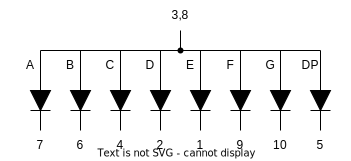
\includegraphics[width=0.5\textwidth]{./txt/image.png}
  \caption{ファイルが存在するときの実行結果}
  % \label{fig:result_pr1_dup}
\end{figure}
\newpage
\input{./txt/tower.txt}
\section{考察}
\subsection{スタックの実装}
スタックの実験結果より、満杯のスタックにさらにpushしようとしたときにエラー表示となり中身を壊すことなく処理を終えることが出来ている。また、中身がないときにpopしようとしてもエラーが出力されている。
このことからスタックの基本的な動作が期待通りに行われていることがわかる。
\subsection{ハノイの塔}

\section{付録:今回使用したプログラム}
\lstinputlisting[caption={stack.c}, label={lst:stack.c}]{stack.c}
\lstinputlisting[caption={tower.c}, label={lst:tower.c}]{tower.c}


\end{document}